\documentclass[Rapport/Rapport_main.tex]{subfiles}
\begin{document}
\subsection{Hardware Arkitektur}
Der vil i de følgende afsnit beskrives hardware arkitekturen for Beer Pong bordet. Hardware arkitekturen illustreres ved brug af Block Definitions Diagrams(BDD), hvor der hertil laves en beskrivelse af blokkene. Derefter laves et Internt Block Diagram (IBD) til at vise grænseflader og interne forbindelser i blokken. I de følgende diagrammer vil der være blokke markeret med \textbf{grøn} og \textbf{orange}. De \textbf{grønne} blokke er indkøbte blokke, der ikke er blevet modificeret på anden vis. De er blevet indkøbt af den grund, at udviklingen af disse komponenter ikke prioriteres i projektet. De \textbf{orange} blokke er også indkøbte komponenter, men her er komponenterne modificeret med egen software.
\subsubsection{Overordnet Hardware Arkitektur}
Den overordnede hardwarearkitektur kan ses i et BDD for Beer Pong bordet i figur \ref{fig:rap_overall_hardware_bdd}.

\begin{figure}[H]
    \centering
    \makebox[\textwidth][c]{%
        \includegraphics[width=1.3\columnwidth,trim={0.24in 0.24in 0.24in 0.24in},clip, page=2]{Arkitektur/graphics/BDD_og_IBD.pdf}
    }
    \caption{Overordnet blok definitionsdiagram for systemet.}
    \label{fig:rap_overall_hardware_bdd}
\end{figure}
Af figuren ses Display'et, som værende markeret med grøn, da denne blok er indkøbt.\\
Tilhørende laves der et IBD for det overordnede system, hvilket ses i figur \ref{fig:rap_overall_hardware_ibd}.

\begin{figure}[H]
    \centering
    \makebox[\textwidth][c]{%
        \includegraphics[width=1.3\columnwidth,trim={0.24in 0.24in 0.24in 0.24in},clip, page=5]{Arkitektur/graphics/BDD_og_IBD.pdf}
    }
    \caption{Overordnet intern blokdiagram for systemet.}
    \label{fig:rap_overall_hardware_ibd}
\end{figure}
IBD'et i figur \ref{fig:rap_overall_hardware_ibd} viser som sagt de interne forbindelser i systemet. Det vigtige at observere på IBD'et er kommunikationen mellem RPi (master) og de to Player sides og Ball dispenser (slaver). Her bruges der som beskrevet i analysen \fullref{analyse:sec:comm_analyse} I2C. En ulempe ved I2C er at det altid er masteren som skal initiere kommunikationen. Det vil kræve at den hele tiden skal polle oplysninger fra slaverne for fx. at få oplysninger hvornår der indsættes en mønt. Dette anses som værende upraktisk. Derfor tilføjes der for hver slave en interruptlinje,  som slaven trækker lav når den har information den vil videregive til masteren/RPi. Disse interruptslinjer er ligesom signalerne for I2C protokollen open-drain. Dette gøres for at der kan håndteres kommunikation mellem et 3.3V system og et 5V system. Til dette kræves der pull-up modstande som beskrives i  \\
Nu hvor systemet er beskrevet overordnet, så kan der gås lidt mere i dybden med de enkelte blokke.
\subsubsection{Playerside - Hardware Arkitektur}
Til at starte med kigges der på Hardware arkitekturen for Playerside. Til at få overblik over de blokke som Playerside består af, laves et BDD der kan ses på figur \ref{fig:rap_playerside_hardware_bdd}.

\begin{figure}[H]
    \centering
    \makebox[\textwidth][c]{%
        \includegraphics[width=1.3\columnwidth,trim={0.24in 0.24in 0.24in 0.24in},clip, page=3]{Arkitektur/graphics/BDD_og_IBD.pdf}
    }
    \caption{Blok definitionsdiagram for Player side.}
    \label{fig:rap_playerside_hardware_bdd}
\end{figure}
Kigges der på BDD'et så ses det, at \textsc{Power Supply} er indkøbt og derfor ikke udarbejdet i projektet.\\
Playerside består af 6 \textsc{Cup Holder}, der hver især består af \textsc{Cup light} og \textsc{Cup sensor}. CupHolder sørger altså for lyset og detektering af \textit{Game Events}.\\ 
Der skal også være en \textsc{Cup Holder Controller}, som styrer lyset på samtlige \textsc{Cup Holders} og samler og filtrerer sensor signalet fra samtlige \textsc{Cup Holders}. \\ 
Til sidst er der indkøbt en PSoC Player Side, som er en PSoC 5LP Dev kit\cite{psoc5lp}, hvor der er implementeret softwaren PlayerSideApp på. Derfor er blokken orange. Denne blok behandler sensor outputtet fra \textsc{Cup Holder Controller} og styrer lyset gennem \textsc{Cup Holder Controller}.\\
De interne signaler for Playerside kan ses i IBD'et i figur \ref{fig:rap_playerside_hardware_ibd}.
\begin{figure}[H]
    \centering
    \makebox[\textwidth][c]{%
        \includegraphics[width=1.3\columnwidth,trim={0.24in 0.24in 0.24in 0.24in},clip, page=6]{Arkitektur/graphics/BDD_og_IBD.pdf}
    }
    \caption{Intern blokdiagram for Player side.}
    \label{fig:rap_playerside_hardware_ibd}
\end{figure}
De fulde blok- og portbeskrivelser kan ses i \textbf{Arkitektur} dokumentet afsnit \fullref{arch:sec:playerside_hardware_block_description}

\subsubsection{Ball dispenser - Hardware Arkitektur}
Det næste der kigges på er hardware arkitekturen for Ball dispenser. Denne blok findes der kun en af i systemet og BDD'et for delsystem ses i figur \ref{fig:rap_balldispenser_hardware_bdd}.
\begin{figure}[H]
    \centering
    \makebox[\textwidth][c]{%
        \includegraphics[width=1.3\columnwidth,trim={0.24in 0.24in 0.24in 0.24in},clip, page=4]{Arkitektur/graphics/BDD_og_IBD.pdf}
    }
    \caption{Blok definitionsdiagram for Ball dispenser.}
    \label{fig:rap_balldispenser_hardware_bdd}
\end{figure}
Det ses af figur \ref{fig:rap_balldispenser_hardware_bdd}, at Ball dispenser består af en \textsc{Coin Collector}, hvor der indkastes en mønt, der detekteres af en sensor og behandles af en motor. Hvis den rigtige mønt er indkastet, så står \textsc{Ball release} for at dispensere bolde, hvilket gøres med en motor. Til begge motorer hører en \textsc{Motor controller} til at styre motoren. Ball dispenser skal også opdatere \textsc{Status LEDs} i forhold til om der mangler bolde eller dispenseren er fuld. Dette detekteres desuden med \textsc{Ball count sensor}. Af figuren ses det også at \textsc{Power Supply}, \textsc{Motor}, \textsc{Motor controller} og \textsc{PSoC ball dispenser} er indkøbt, hvor \textsc{PSoC ball dispenser} anvender egen software, BallDispenserApp.\\
De interne signaler i blokken kan desuden ses i figur \ref{fig:rap_balldispensere_hardware_ibd}.

\begin{figure}[H]
    \centering
    \makebox[\textwidth][c]{%
        \includegraphics[width=1.3\columnwidth,trim={0.24in 0.24in 0.24in 0.24in},clip, page=7]{Arkitektur/graphics/BDD_og_IBD.pdf}
    }
    \caption{Intern blokdiagram for Ball dispenser.}
    \label{fig:rap_balldispensere_hardware_ibd}
\end{figure}

Blokbeskrivelser og portbeskrivelser for Ball dispenser kan ses i \textbf{Arkitektur} dokumentet i afsnit \fullref{arch:sec:balldispenser_hardware_ports}.

\subsubsection{RPi - Hardware Arkitektur}
RPi er hjernen i systemet, der er derfor ikke mange hardware blokke, der hører til her, da det meste er logik lavet i software. BDD'et for RPi kan ses i figur \ref{fig:rap_rpi_hardware_bdd}.
\begin{figure}[H]
    \centering
    \makebox[\textwidth][c]{%
        \includegraphics[width=1\columnwidth,trim={0.24in 0.24in 0.24in 0.24in},clip, page=9]{Arkitektur/graphics/BDD_og_IBD.pdf}
    }
    \caption{Blok definitionsdiagram for RPi.}
    \label{fig:rap_rpi_hardware_bdd}
\end{figure}
Figur \ref{fig:rap_rpi_hardware_bdd} viser at \textsc{RPi Power Supply} , samt en \textsc{RPi Zero W} er indkøbt, hvor der på RPi'en er udviklet egen softwaren til anvendelse i systemet, nemlig RPiApp. Den eneste egentlige hardware blok er \textsc{Pull up resistors}, der er de resistorer der anvendes til interrupts fra de andre delsystemer. Det er vigtigt at det er pull-up modstande til 3.3V og ikke 5V. Det er ikke nødvendigt med pull-up modstande til I2C signalerne, da RPi Zero W allerede har interne pull-up modstande \autocite{RPiPins}  \\
De interne signaler for denne blok kan ses i figur \ref{fig:rap_rpi_hardware_ibd}.
\begin{figure}[H]
    \centering
    \makebox[\textwidth][c]{%
        \includegraphics[width=1.3\columnwidth,trim={0.24in 0.24in 0.24in 0.24in},clip, page=10]{Arkitektur/graphics/BDD_og_IBD.pdf}
    }
    \caption{Intern blokdiagram for RPi.}
    \label{fig:rap_rpi_hardware_ibd}
\end{figure}
Blokbeskrivelser for RPI kan ses i \fullref{arch:sec:rpi_hardware_block_description} og de fulde portbeskrivelser kan ses i afsnit \fullref{arch:sec:RPi_hardware_ports} af i \textbf{Arkitektur} dokumentet. 


\end{document}